
\documentclass[a4paper,UKenglish,cleveref, autoref, thm-restate]{tgdk-v2021}
%This is a template for producing TGDK articles. 
%See tgdk-v2021-authors-guidelines.pdf for further information.
%for A4 paper format use option "a4paper", for US-letter use option "letterpaper"
%for british hyphenation rules use option "UKenglish", for american hyphenation rules use option "USenglish"
%for section-numbered lemmas etc., use "numberwithinsect"
%for enabling cleveref support, use "cleveref"
%for enabling autoref support, use "autoref"
%for anonymousing the authors (e.g. for double-blind review), add "anonymous"
%for enabling thm-restate support, use "thm-restate"
%for enabling a two-column layout for the author/affilation part (only applicable for > 6 authors), use "authorcolumns"
%for producing a PDF according the PDF/A standard, add "pdfa"

%\pdfoutput=1 %uncomment to ensure pdflatex processing (mandatatory e.g. to submit to arXiv)
%\hideTGDK  %uncomment to remove references to TGDK series (logo, DOI, ...), e.g. when preparing a pre-final version to be uploaded to arXiv or another public repository

%\graphicspath{{./graphics/}}%helpful if your graphic files are in another directory
\usepackage{graphicx}
\usepackage{booktabs}
\usepackage{pgfplots}
\usepgfplotslibrary{groupplots}
\pgfplotsset{compat=1.18}
\usepackage{amsmath}
\usepackage{amssymb} 
\usepackage{hyperref}
\usepackage{placeins}
\usepackage{xcolor}
% More permissive float placement: the results section carries several large tables
\renewcommand{\topfraction}{0.9}
\renewcommand{\bottomfraction}{0.8}
\renewcommand{\textfraction}{0.07}
\renewcommand{\floatpagefraction}{0.75}
\setcounter{topnumber}{3}
\setcounter{totalnumber}{5}

\usepackage[linesnumbered,ruled,vlined]{algorithm2e}
\bibliographystyle{plainurl}% the mandatory bibstyle

\title{Extending Mined Rules for Link Prediction with Schema-based Exceptions}

%\titlerunning{Dummy short title} %TODO optional, please use if title is longer than one line

\author{Giacomo {Zamprogno}\footnote{Corresponding author}}{Vrije Universiteit Amsterdam, The Netherlands \and Hybrid Intelligence Consortium, The Netherlands}{g.zamprogno@vu.nl}{https://orcid.org/0009-0009-6474-1987}{This  work  is  supported  by  the  Hybrid  Intelligence  programme (https: //www.hybrid-intelligence-centre.nl/), funded  by  a  10-year  Zwaartekracht  grant  from  the  Dutch Ministry of Education, Culture and Science (NWO).}%TODO mandatory, please use full name; only 1 author per \author macro; first two parameters are mandatory, other parameters can be empty. Please provide at least the name of the affiliation and the country. The full address is optional. Use additional curly braces to indicate the correct name splitting when the last name consists of multiple name parts.

\author{Ilaria Tiddi}{Vrije Universiteit Amsterdam, The Netherlands \and Hybrid Intelligence Consortium, The Netherlands}{i.tiddi@vu.nl}{https://orcid.org/0000-0001-7116-9338}{}

\author{Bart Verheij}{University of Groningen, The Netherlands \and Hybrid Intelligence Consortium, The Netherlands}{Bart.Verheij@rug.nl}{https://orcid.org/0000-0001-8927-8751}{}

\author{Stefan Schlobach}{Vrije Universiteit Amsterdam, The Netherlands \and Hybrid Intelligence Consortium, The Netherlands}{k.s.schlobach@vu.nl}{https://orcid.org/0000-0002-3282-1597}{}

\authorrunning{G. Zamprogno, I. Tiddi, B. Verheij and S. Schlobach} %TODO mandatory. First: Use abbreviated first/middle names. Second (only in severe cases): Use first author plus 'et al.'

\Copyright{Giacomo Zamprogno, Ilaria Tiddi, Bart Verheij and Stefan Schlobach} %TODO mandatory, please use full first names. TGDK license is "CC-BY";  http://creativecommons.org/licenses/by/4.0/

\ccsdesc[100]{\textcolor{red}{Computing methodologies~Artificial intelligence~Knowledge representation and reasoning}} %TODO mandatory: Please choose ACM 2012 classifications from https://dl.acm.org/ccs/ccs_flat.cfm 

\keywords{Knowledge Graphs, Link Prediction, Rule Mining, Non-monotonic Reasoning} %TODO mandatory; please add comma-separated list of keywords

\category{} %optional, e.g. invited paper

\relatedversion{} %optional, e.g. full version hosted on arXiv, HAL, or other respository/website
%\relatedversiondetails[linktext={opt. text shown instead of the URL}, cite=DBLP:books/mk/GrayR93]{Classification (e.g. Full Version, Extended Version, Previous Version}{URL to related version} %linktext and cite are optional

%\supplement{}%optional, e.g. related research data, source code, ... hosted on a repository like zenodo, figshare, GitHub, ...
%\supplementdetails[linktext={opt. text shown instead of the URL}, cite=DBLP:books/mk/GrayR93, subcategory={Description, Subcategory}, swhid={Software Heritage Identifier}]{General Classification (e.g. Software, Dataset, Model, ...)}{URL to related version} %linktext, cite, and subcategory are optional

%\funding{(Optional) general funding statement \dots}%optional, to capture a funding statement, which applies to all authors. Please enter author specific funding statements as fifth argument of the \author macro.

%\acknowledgements{I want to thank \dots}%optional

%\nolinenumbers %uncomment to disable line numbering


%EditorialOffice macros (do not touch as author)%%%%%%%%%%%%%%%%%%%%%%%%%%%%%%%%%%%
\Volume{1}
\Issue{1}
\Article{42}
\DateSubmission{Date of submission}
\DateAcceptance{Date of acceptance}
\DatePublished{Date of publishing}
\SectionAreaEditor{TGDK section area editor}
%%%%%%%%%%%%%%%%%%%%%%%%%%%%%%%%%%%%%%%%%%%%%%%%%%%%%%%%%

\begin{document}

\maketitle

%TODO mandatory: add short abstract of the document
\begin{abstract}
Link Prediction (LP) is the task of expanding information in Knowledge Graphs (KGs) by suggesting new relations between their entities. Mining and applying inference rules for this task can be used, with competitive performance, to maintain transparency with respect to machine learning methods for LP, which behave as black-boxes. These rule-based methods suffer from a lack of expressivity and  rarely leverage semantic information of the KG, using instead only entity-level triples and leading to inconsistencies when considering the KG schema restrictions.
In this work, we propose to extend rule expressivity with non-monotonicity. In particular, we leverage KG schema information to extend the mined rules with exception cases, in order to make the KG more consistent and semantically accurate. We automatically define exception cases based on the predicted relations, pruning the search space  when the rule could produce semantically incorrect facts, based on the commonly present restrictions of functionality, domain and range. 
We compare our approach with the baselines from two rule-miners (AMIE3, AnyBURL) and on four large-scale KGs representing varying domains and curation levels, assessing how they perform with both standard rank-based LP metrics and semantic-aware metrics. We also show the method can work on inverse functionality, via ad ad-hoc modified dataset, as common benchmark rarely include the restriction.  
Our results suggest that while the semantic quality of mined rules varies widely between different rule miners and datasets, inconsistencies are generated in most cases, regardless of KG size and schema complexity. Further, we show that applying exceptions at single-rule level (thus ignoring between-rule interactions) allows to substantially reduce the number of inconsistent triples in all cases, at the cost of a limited increase in inference time. We finally report that rank-based LP metrics are influenced by the differences in rule expressivity in a limited way, further suggesting the need for  metrics that can take into account the semantic quality of the predicted triples.
\end{abstract}

\section{Introduction}
In recent years, Knowledge Graphs (KGs) \cite{hogan_knowledge_2022} have attracted interest due to  being inherently readable by both humans and machines, allowing  to encode expert knowledge and to be easily processed algorithmically. Their usage spans from industrial applications \cite{deng_research_2022,han_construction_2022,tang_exploring_2023} to shareable scientific repositories \cite{dessi_cs-kg_2025,himmelstein_systematic_2017,jaradeh_open_2019}, and, with the recent rise of Large Language Models, they have been applied as means to ground the generative process with reliable facts \cite{procko_graph_2024}. Despite this, KGs are often incomplete, meaning that they do not, and often cannot, capture all the facts relevant to their domain fields: they can miss information about individuals, or relations that connect them. KG incompleteness stems not only from imperfections in data extraction and expert curation, but also from the fact that new knowledge is  regularly discovered. The task of KG completion aims at addressing such incompleteness. \\
\indent A specific approach to KG completion is Link Prediction (LP), which aims at predicting missing links (i.e. edges) that are likely to be true in the context of the KG. Recently, Rule Mining (RM)~\cite{harth_fast_2020,meilicke_anytime_2024} has gained renewed interest in Link Prediction, showcasing competitive performance w.r.t. subsymbolic, black-box, methods such as KG embeddings \cite{wang_knowledge_2017} and Graph Neural Networks \cite{ye_comprehensive_2022}, while maintaining human-readability. These methods usually involve extracting patterns in the data, which usually take the shape of paths connecting pairs of entities -- e.g. the rule  $\texttt{(X,childOf,Y)},$ $ \texttt{(Y,bornIn,C)} \rightarrow \texttt{(X,bornIn,C)}$ suggests that a child X is often born in the same city C as a parent Y. \\
\indent  Despite being closer to symbolic methods, RM algorithms often fail to leverage the semantic information that might come with the KG, focusing instead on frequent patterns. 
Following the previous example, given query \texttt{(virginiaWoolf, bornIn,?)}, the rule presented above will be applied for two matching bodies, materializing two new triples, as the parents are born in two different cities (London and Calcutta, as Virgina Woolf's parents were born in different cities). This would be inconsistent given the functionality property (i.e. having at most one object value for each subject x) of `bornIn'. This is only partially captured by standard LP metrics, which are computed from a ranking of predictions given a test set \cite{paulheim_knowledge_2016}. In other words, the ranking of the predictions might be influenced by the number of predictions, but a standard metric will not highlight the issue with the inconsistency (a person cannot have two birth cities). This is likely to reduce the applicability of LP solutions in practical cases: while inconsistent triples from the same rule might have a limited effect on ranking metrics, they require repairing the knowledge base.\\
\indent In this work, we tackle the problem of maintaining consistency via a non-monotonic approach, operating under the hypothesis that integrating exceptions into rules increases granularity and preempts inconsistencies. Similar methods have been previously proposed \cite{gad-elrab_exception-enriched_2016,lisi_combining_2017,tran_towards_2017}, but they typically derive exceptions by refining rule sets based solely on data distribution, leaving the semantic layer unaddressed. Our approach is instead \textit{focused on the information present in ontological schemas of KGs.} Specifically, given a set of semantic restrictions and a mined rule set, our approach automatically appends relevant exception conditions to the rules. These conditions act as a safeguard during the application phase, preventing the triggering of rules that would result in trivial violations of the ontology. We then compare the semantic validity of triples predicted by the original and extended rule sets to evaluate the trade-off involved in preventing trivial rule-based violations. This comparison is conducted on four large-scale KGs representing varying domains and curation levels: YAGO4.5, a general-purpose KG derived from Wikidata with a highly curated schema based on schema.org; NELL995, an automatically generated KG with a rigid, ad-hoc schema; Hetionet, a domain-specific KG featuring a smaller, high-level ontology and CSKG2.0, collecting statements from millions of Computer Science papers, automatically populated using a granular, expert validated, ontology. We further show how our method is also applicable on the less widely available restriction of inverse-functionality, on an adapted version of the YAGO dataset.\\
\indent In our results, we analyze our method applied to two baselines rule miners, for each considering two different types of rule sets and their non monotonic extensions. Our results show that the semantic accuracy of the mined rules varies substantially when changing the quality of the input KG, its curation level and the complexity of the rule set. Nonetheless, we show that applying exceptions at single-rule level (i.e. without considering between-rule interaction)  results in a decrease in the number of inconsistent triples predicted with a limited increase in computational time in all datasets.
Additionally, we notice that rank-based metrics tend to be influenced by the exceptions in either a non-significant or a negative way, revealing the need for integrating such metrics with more semantic-oriented evaluations.

\section{Related Work}

\subsection{Link Prediction approaches}
Link Prediction is a widely studied task and has been tackled with multiple approaches, most notably KG embeddings (KGEs), Graph Neural Networks (GNNs) and Rule Mining. 

KGEs involve mapping the entities and relations of the KG into a lower-dimensional vector representations. Methods such as~\cite{bordes_translating_2013,trouillon_complex_2016, sun_rotate_2019} usually learn the vectors' weight by minimizing a loss over a scoring function that is intended to preserve certain properties of the inner geometric structure of the KG. Similarly, GNNs (e.g., \cite{kipf_semi-supervised_2016,zeb_complex_2022}) are subsymbolic approaches that learn a vectorized representation of the graph, but they are usually deeper and also embed information about node features and neighborhood via message passing. In general, models in both these classes tend to be black-box like, thus lacking interpretability. For an in-depth analysis of the state-of-the-art methods (with a few examples for alternatives to tackle the mentioned downsides), we refer to \cite{arrar_comprehensive_2024}.

\subsection{Rule Mining}
Rule Mining \cite{zeng_logical_2023} involves the discovery of symbolical rules (typically Horn-like) from the data, which holds the promise of being more interpretable and is the focus of this work. In Section \ref{sec:exp} we generated rule sets using AnyBURL \cite{meilicke_anytime_2024} and AMIE3 \cite{harth_fast_2020}, which respectively employ path sampling (bottom-up) and systematic generation and testing (top-down) with pruning heuristics.
Other rule miners have been proposed: \cite{pirro_relatedness_2020} uses a T-box based approach to suggest rule candidates, and SAFRAN \cite{ott_safran_2021} is an extension of AnyBURL using noisy-or, where the confidence of a predicted triple is an aggregation of the confidence of all relevant rules, once redundant rules are removed. 
%We currently do not use noisy-or, as it would require exploring the interplay between rule redundancy and exceptions, but we intend to apply this in the future. 
We refer to \cite{wu_rule_2023} for an extended analysis of rule learning methods which we do not include in this work: specifically, beyond our analyzed methods, it includes a survey of deep-learning-based methods for RM . For the scope of this paper, we focused on the most directly interpretable and tunable models, but we consider the set of mined rules as an input for our analysis, so any of the reviewed methods should in principle be applicable.

\subsection{Non-monotonic approaches to Knowledge Graphs and Link Prediction}

Non-monotonicity has been applied in knowledge representation as a way to handle defeasible knowledge, and a substantial body of work exists on the topic of defeasible description logics \cite{britz_principles_2020} or integrating rules with ontologies under non-monotonic semantics \cite{eiter_combining_2008}. Our work takes a more operationalized stance, as we do not focus on formal entailment and semantics, but we use semantic consistency as a means to prune rules during KG completion and materialization.

Similar to our setting, there exists a line of work that learns exceptions from the data. \textit{Exception-enriched rule learning}~\cite{gad-elrab_exception-enriched_2016} also starts from an input rule-set, and revises them into rules of the form $body \wedge not\ E(X) \rightarrow head$, where the candidate exception predicates are drawn from \textit{exception witness sets} -- predicates whose presence correlates with the rule failing on the KG. This was further extended in expressivity~\cite{tran_towards_2017}, and framed more generally as an inductive logic programming~\cite{muggleton_inductive_1991} problem over KGs~\cite{lisi_combining_2017}.                                         

While inspired from this, our approach differs in two ways. First, rather than inferring the exceptions from the distribution of the data, we derive them from the ontological restrictions, so exceptions are guaranteed to represent inconsistencies in the materialized graph. Second, we apply exceptions at rule materialization, not rule learning, allowing our method to be agnostic (fixed the rule's linguistic bias) to the rule miner.
% Non-monotonic extensions of rule-sets have previously been proposed. A series of studies \cite{gad-elrab_exception-enriched_2016,lisi_combining_2017,tran_towards_2017} explores learning exceptions via an inductive logic programming \cite{muggleton_inductive_1991} approach, while we aim at exploiting ontological information. 

\subsection{Schema integration in Link Prediction}
Finally, using T-box or ontological knowledge to improve Link Prediction has been the subject of study of various neuro-symbolic approaches.
Schemas have been used to improve the training signal: type restrictions can constrain the generation of negative samples~\cite{krompas_type-constrained_2015,jain_improving_2021}, or be included in the loss function to penalize domain/range violations \cite{hubert_treat_2024}. Other methods operate at the representation level, and embed the schema together with the triples, either by jointly modeling entity-concept associations~\cite{hao_universal_2019}, or by constructing geometric models of the the description logic axioms~\cite{kulmanov_embeddings_2019}. In the symbolic setting, schema information has been used at rule learning time, either to type the mined rules~\cite{wu_learning_2022} or to drive the generation of rule candidates~\cite{pirro_relatedness_2020}. Finally, a fourth group places the schema in an iterative loop, alternating rule mining and embedding learning and retaining only schema correct triples between iterations~\cite{wiharja_schema_2020,zhang_iteratively_2019}.





% \cite{jain_improving_2021} and 
% \cite{hubert_treat_2024} use schema-based inconsistencies to generate negative samples for KGEs or to directly operate in the training loss, \cite{wu_learning_2022} include type information in the rule learning process, \cite{wang_schema-aware_nodate,wiharja_schema_2020} focus on \textit{schema correct} triples to iteratively learn LP methods alternating rule mining and KGEs learning and \cite{hao_universal_2019} enhances embedding by including the entity-concept associations in the learning

%\subsection{Repairs}

\section{Problem Definition}
In this section, we first describe the basic terminology, and then introduce the research problem we aim to tackle.

\subsection{Terminology}
Our input is defined as a tuple $(\mathcal{G},\mathcal{O},\mathcal{IR})$ where:
\begin{itemize}
    \item $\mathcal{G}$ is a Knowledge Graph: $$\mathcal{G} = (\mathcal{E}, \mathcal{R}, \mathcal{T})$$ where $\mathcal{E}$ is the (finite) set of entities (nodes), $\mathcal{R}$ is the (finite) set of relation types, and $\mathcal{T} \subseteq \mathcal{E} \times \mathcal{R} \times \mathcal{E}$ is the set of known triples (edges). From the example of the previous section, \texttt{(virginiaWoolf,childOf,leslieStephen)}, \texttt{(leslieStephen,bornIn,London)} are facts in the KG.
    \item $\mathcal{O}$ is a set of ontological restrictions, defined in a given Description Logic formalism. \texttt{(bornIn, subPropertyOf, FunctionalProperty)} is an example of such restriction.
    \item $\mathcal{IR}$ is a set of inference rules of the type $$\bigwedge_{i=0}^{n} (S_i, b_i, O_i) \rightarrow (X, h , Y)$$ where $X,Y \in \{S_i\}\cup{\{O_i\}}$, $b_i,h \in \mathcal{R}$ and $S_i,O_i$ are interpreted as variables to be grounded with elements of $\mathcal{E}$ such that given a variable substitution $\theta$, $(S_i, b_i, O_i)_{/\theta} \in \mathcal{G}$.     
\end{itemize}
In the specific scenario we consider, the substitution requires each variable to get a distinct grounding, i.e. $S_{i/\theta} \not= S_{j/\theta}\quad\forall \quad i \not=j$ and $S_{i/\theta} \not=O_{j/\theta}\quad if\quad S_i \not=O_j$.

    $\mathcal{IR}$ can be also seen as \textit{Horn rules}, i.e. of the type $B \rightarrow H$, where $B$ is a conjunction of atoms and $H$ is a single atom. In this work, we consider atoms as being \textit{triple patterns} of the type $(V1,p,V2)$, where the relation is known, while subject and objects are variables.

    Following the example, $\texttt{(X,childOf,Y)}, \texttt{(Y,bornIn,C)} \rightarrow \texttt{(X,bornIn,C)}$ is an example of such rule, the body can be grounded by \\$\theta:$ \texttt{(X=virginiaWoolf,Y=leslieStephen,C=London)}, and would predict the head: \\$\texttt{(virginiaWoolf,bornIn,London)}$.


\subsection{Link Prediction}
Link Prediction  refers to the task of predicting missing links in the graph. More precisely, the goal is to infer plausible triples $\texttt{(s,r,o)}$ that are not present in $\mathcal{T}$ but are likely to hold.

LP is usually tested via the \textit{silver-standard} method: a set of triples from the original graph is removed, and the LP methods are tasked to rank each removed triple with respect of its possible corruptions (random substitutions of its components), where ideally the test triple is ranked among the most likely ones. 
In the context of Rule Mining for Link Prediction, most rule-sets $\mathcal{IR}$ assign a \textit{confidence} value to each rule. So, given a test triple $\texttt{(s,r,o)}$, all rules that allow to infer $\texttt{(s,r,?)}$ are queried, ranking the predicted $\texttt{(s,r,o')}$ by an aggregation of the confidence scores of the rules which can correctly predict each triple. The same can be done for $\texttt{(?,r,o)}$ ranking predicted $\texttt{(s',r,o)}$.

\subsection{Rule Mining}

Rule Mining (RM) is the task of constructing a set of inference rules, typically of the Horn type (B→H), each associated with a measure of its quality.

A specific and common type is the Closed Rule (CR), which is a rule where every atom appears, often expressed as a sequence of the type: $$\bigwedge_{i=1}^{n} (A_{i-1}, b_i, A_i) \rightarrow (A_0, h , A_n)$$ 
These are considered relatively easy to mine as they involve looking for closed paths within the graph structure.

Central to mining and materializing these rules is the concept of \textit{grounding}: a grounding  is a variable substitution $\theta$ that maps a given triple pattern $\text{tp}: (V1, p, V2)$, into a syntactically correct triple, i.e. both V1 and V2 are mapped to elements of $\mathcal{E}$.
    % the triple $tp_{/\theta}: (v1, p, v2) $ resulting from applying the variable substitution, is such that $tp_{/\theta} \in \mathcal{G}$
In the following section, we refer to body groundings (resp. Head Grounding) as a variable substitutions $\theta$ for which all triple patterns in the body (head) respectively, are grounded. A notion of \textit{confidence} is attached to each rule, computed as the ratio between groundings that satisfy both head and body, and all possible groundings of the body, given the training data.
    
\subsection{Semantic Consistency of a KG and Violations}

In general, a KG is consistent if $\mathcal{G} \cup \mathcal{O} \not\models \bot$. 

Assuming a consistent KG as an input, given a set of inference rules $IR$, it might still be the case that $\mathcal{G}^{IR} \cup \mathcal{O} \models \bot$. We define three ways in which rules can lead to inconsistencies:

\begin{itemize}
    \item \textit{in-graph violation}: in-graph violations are inconsistencies derived by data already present in the graph when a rule conclusion is materialized.
    \item \textit{in-rule violation}: we define in-rule violations as inconsistencies caused by one or more conclusions materialized from a given rule. 
    \item \textit{out-rule violation}: comparatively, out-rule violations are inconsistent conclusions predicted using different rules.
\end{itemize}

Examples with the functional property restriction:
\begin{itemize}
    \item \textit{in-graph violation} : a given \texttt{(s,r,o)} conclusion would violate information already in the graph:  $\texttt{(X,childOf,Y)}, \texttt{(Y,bornIn,C)} \rightarrow \texttt{(X,bornIn,C)} $ might derive that a person \texttt{personx} is born in the same city \texttt{cityp} of their parents, even if the graph already contains a \\ $\texttt{(personx, bornIn, city2)}$ triple, where \texttt{cityp} and \texttt{city2} are distinct.
    \item \textit{in-rule violation}: the same rule for a given \texttt{(s,p,?)} query might get two or more different conclusions: $\texttt{(X,childOf,Y)}, \texttt{(Y,bornIn,C)} \rightarrow \texttt{(X,bornIn,C)} $, in the case of parents being born in different cities, two head triples will be derived, which will generate an inconsistency.
    \item \textit{out-rule violation}: two different rules can trigger for a given query\\ \texttt{(s,p,?)}: 
    $\texttt{(X,childOf,Y)}, \texttt{(Y,bornIn,C)} \rightarrow \texttt{(X,bornIn,C)} $ and\\ $\texttt{(X,livesIn,C)} \rightarrow \texttt{(X,bornIn,C)}$. Both rule bodies can apply, possibly resulting in the prediction of inconsistent conclusions.
\end{itemize} 

\subsection{Research Question}

Given our problem definition, we intend to tackle the issue of the semantically-inconsistent materialization of rule sets for LP by integrating knowledge about the schema restrictions. 
% As computing \textit{out-rule} violations would involve a computationally complex analysis, possibly requiring to materialize a large number of them for each candidate, in this work we focus on removing \textit{in-graph} and \textit{in-rule} violations. 
We focus on removing \textit{in-graph} and \textit{in-rule} violations -- we leave computing \textit{out-rule} violations for future work, since they would require to materialize a large number of violations for each candidate at high computational costs. Our research question is as follows: 

\textit{\textbf{RQ:}To what extent does automatically extending LP rule sets with schema-based exceptions that eliminate in-rule and in-graph conflicts reduce inconsistencies in predicted triples, and how does this integration affect predicting performance and computational efficiency?}

\section{Non-monotonic Extension of Rules}
In the following sections we will present the approach we propose to answer the research question. We focus on the effect of removing in-rule and in-graph violations by extending the original $\mathcal{IR}$ non-monotonically, i.e. by defining exception patterns that, if matched, will stop the application of the rule\footnote{Our algorithm, and evaluation settings, can be found at the following repository: \url{https://github.com/Zamprognog/NMRuleExtension.git}.}. 


\subsection{Approach} \label{sec:approach}
\subsubsection{Schema-based Exceptions} Given $\{\mathcal{G,IR,O}\}$ we generate $\mathcal{IR}^{nm}$, a non-monotonic extension of the rule set, where the exceptions are sufficient conditions for in-rule and in-graph violations. Table \ref{tab:ijp} collects the list of inconsistency patterns adapted given the set of property restrictions we focus on: domain, range, functionality and
inverse functionality. 

\subsubsection{Materializing with Exceptions} Algorithm \ref{alg:materialize} illustrates the materialization of $\mathcal{G}^{IR^{nm}}$, for each rule \textit{$r_i$}, given input $\{\mathcal{G,IR,O}\}$:
\begin{itemize}
    \item We iterate over candidates $e \in \mathcal{E}$ as a substitution of the first variable $X$ of \textit{$r_i$}.
    \item If in-graph exceptions are violated, further search for the remaining variables is halted (6-9).
    \item A path is searched from $e$ with a recursive depth-first search (DFS) in order to find a valid $\theta$ (10). If $\exists \theta: body(r)_{/\theta} \in \mathcal{G}$ ,  $head(r)_{/\theta} \not\in \mathcal{G}$ and $\mathcal{G} \cup \mathcal{O} \not\models exception(r)_{/\theta}$, the algorithm proceeds and $head(r)_{/\theta}$ is added to $\mathcal{G}^{IR^{nm}}$(11,16).
    \item Otherwise, the specific rule activation is skipped (12-14).  
\end{itemize}

Following \cite{meilicke_anytime_2024}, we implement this strategy as a DFS approach. Similarly to them, we require different variables to have different groundings (concept known as `object identity'). 
%%%%%%%%%%%%%%%%%%
% Pseudocode
%%%%%%%%%%%%%%%%%%%

\newcommand{\GIRnm}{\mathcal{G}^{IR^{nm}}}
\newcommand{\G}{\mathcal{G}}
\newcommand{\E}{\mathcal{E}}
\newcommand{\Oset}{\mathcal{O}}

% \vspace{1em}
\begin{algorithm}[t]
\SetAlgoLined
\DontPrintSemicolon
\SetKwInOut{Input}{Input}
\SetKwInOut{Output}{Output}
\SetKw{Break}{break}

\Input{Graph $\G$, Set of Rules $R$, Candidates $\E$, Ontology $\Oset$}
\Output{Materialized Graph $\GIRnm$}

\BlankLine
Initialize $\GIRnm \leftarrow \G$\;
\BlankLine

\ForEach{rule $r_i \in R$}{
    \ForEach{candidate $e \in \E$}{
        \BlankLine
        $valid \leftarrow True$\;
        $possiblePredictions \leftarrow \emptyset$\;
        \BlankLine
        
        \If{in-graph violation detected for $e$}{
            $valid \leftarrow False$\;
            \textbf{continue}\;
        }
        
        \BlankLine
        \ForEach{substitution $\theta$ found via DFS($r_i$, start=$e$)}{
            \BlankLine
            \If{$body(r_i)_{/\theta} \subseteq \G$ \textbf{and} $head(r_i)_{/\theta} \notin \G$}{
                \BlankLine
                \eIf{$\G \cup \Oset \models exception(r_i)_{/\theta}$}{
                    $valid \leftarrow False$\;
                    \Break \tcp*{Halt DFS}
                }{
                    Add $head(r_i)_{/\theta}$ to $possiblePredictions$\;
                }
            }
        }
        
        \BlankLine
        \If{$valid$ \textbf{and} $possiblePredictions \neq \emptyset$}{
            $\GIRnm \leftarrow \GIRnm \cup possiblePredictions$\;
        }
    }
}
\Return{$\GIRnm$}

\caption{Materialize $\mathcal{G}^{IR^{nm}}$}
\label{alg:materialize}
\end{algorithm}
%
%%%%%%%%%%%%%%%%%%
\begin{table}[t]
    \centering
    \caption{Violations  $r: body(r)\rightarrow head(r),head(r) =(A_x, h, A_y)$ assuming a valid substitution $\theta$ for r.}
    \begin{tabular}{|l|l|}
        \hline
        \textbf{Property} & \textbf{Condition for exception} \\
        \hline
        Functional(h)  & $\theta,\theta':A_{x/\theta} =A_{x/\theta'},A_{y/\theta} \neq A_{y/\theta'}, head(r)_{\theta'} \in \mathcal{G} \lor body(r)_{\theta'} \in \mathcal{G}$ \\
        \hline
        Inverse Functional(h) & $\theta,\theta':A_{x/\theta} \neq A_{x/\theta'},A_{y/\theta} = A_{y/\theta'}, head(r)_{\theta'} \in \mathcal{G} \lor body(r)_{\theta'} \in \mathcal{G}$ \\
        \hline
        Domain(h) & $\theta: type(A_{x/\theta}) \sqcap domain(h) \sqsubseteq \bot$ \\
        \hline
        Range(h) & $\theta: type(A_{y/\theta}) \sqcap range(h) \sqsubseteq \bot$  \\
        \hline
    \end{tabular}   
    
    % , in C.W.A. 
    \label{tab:ijp}
\end{table}

\subsubsection{Example}  Let us recall our running example. Given the following triples in the KG: \texttt{(virginiaWoolf, childOf, leslieStephen)}, \texttt{(virginiaWoolf, childOf, juliaStephen)}, \texttt{(leslieStephen, bornIn, London)}, \texttt{(juliaStephen, bornIn, Calcutta)}, \texttt{(virginiaWoolf, almaMater, kingsCollege)}, standard rule mining materialization would activate rule $\texttt{(X,childOf,Y)}, \texttt{(Y,bornIn,C)} \rightarrow \\ \texttt{(X,bornIn,C)}$ and predict both \texttt{(virginiaWoolf, bornIn, London)} and\\ \texttt{(virginiaWoolf, bornIn, Calcutta)}, which are mutually inconsistent. When the schema-based exception for functionality is included, it will trigger once the second grounding is found, stopping any further search. Candidate predictions will be rejected, as the rule is `unsafe', but a lower confidence rule might then apply, e.g. $\texttt{(X,almaMater,U)}, $ $\texttt{(U,locatedIn,C)} \rightarrow \texttt{(X,bornIn,C)}$, which would materialize only the correct triple \texttt{(virginiaWoolf,bornIn,London)}. 
\subsection{Evaluation}
% As our method can currently only work for ungrounded rules, we cannot leverage the full capabilities of the methods, and thus do not aim at strictly improving benchmark metrics, nor intend to perform a direct comparison between models. Our focus is instead on changes in the semantic quality of predicted triples between the monotonic and non-monotonic version of rule sets, the cost in computational time and the residual effect of out-rule violations. Nonetheless, for completeness, we also include results from standard rank-based LP metrics, which should be intended as `validation' against loss of performance between the rule-sets versions, and not as an objective benchmarking result.

% The current limitation of our method to ungrounded rules prevents the leveraging of the full capabilities of the existing techniques. Consequently, we are not focused on strictly improving standard benchmark metrics or conducting a direct comparative analysis between models. 

The goal of our evaluation is to analyze changes in the semantic quality of predicted triples between the monotonic and non-monotonic rule sets, and evaluate the added computational time cost and the residual effect of out-rule violations. Notice that our goal is not to improve benchmark metrics, nor to provide a direct performance comparison of existing rule miners\footnote{Particularly, as later mentioned, we could not use the full expressivity of AMIE (i.e. long rules with constants), due to limitations in computational resources.}. The  standard rank-based LP metrics we  report are used solely for evaluating the different rule set versions and their loss in performance, hence they should not be interpreted as an objective benchmarking result. 

\subsubsection{Materialization evaluation} We rank the rules in descending confidence order and incrementally materialize the predicted triples by applying them on candidate subjects and objects. This process aims at materializing target percentages of the rules (1\%, 5\% and 10\%), but we report the actual number of applied rules too, as it varies from the target either due to all possible heads already being present once the full graph (not only the training set) is considered, and the fact that the semantic exceptions might stop entire rules from producing new triples.\\
\indent The full graph and the newly materialized triples are then both loaded in a triple store (GraphDB \cite{ontotext_graphdb_2024} for speed, and Apache Jena \cite{apache_software_foundation_apache_2024} for run-time evaluation) as separate named graphs. 
For each considered restriction, we then compute the number of new triples that would violate such restriction, as well as the total number of new triples that are inconsistent. This is done via SPARQL queries, which can be accessed in the online repository: we use a RDFS-plus engine, but consider entities as mutually disjoint for functionality matter. We additionally report the computational time to perform the materialization in all conditions.

\subsubsection{Ranking-based LP metrics}
LP metrics are usually \textit{ranking metrics}. Given a set of test triples, i.e. positive triples that we know are in the KG but have not been seen by the model, for each belonging test triple $t_i$ we compute its ranking relative to all possible corruption of its subject and/or object (usually excluding corruptions that would be part of the known graph, known as \textit{filtered} condition).

\begin{itemize}
    \item  Hits@k: 
    \[
    \textit{Hits@}k = \frac{1}{N} \sum_{i=1}^{N} \mathbb{I} \left[ \textit{rank}_i \leq k \right]
    \]
    Where $\mathbb{I}[\cdot]$ equals 1 if condition is true, 0 otherwise.
    \item Mean Reciprocal Rank (MRR): 
    \[
    \textit{MRR} = \frac{1}{N} \sum_{i=1}^{N} \frac{1}{\textit{rank}_i}
    \]
     \item Sem@k:
    \[\textit{Sem}@K = \frac{1}{|\textit{Test}|} \sum_{q \in \textit{Test}} \frac{1}{K} \sum_{t' \in \mathcal{S}_q^K} \textit{consistent}(t',\mathcal{G},\mathcal{O})
    \]
    Where $q$ is a test triple, $\mathcal{S}_q^K$ is the set of ranked top-K predictions for its corruption, and the \textit{consistent} returns true if a given triple is consistent with respect to the KG and related schema, false otherwise. This is an adapted version of the Sem@k metrics ~\cite{hubert_treat_2024}, which checks the number of semantically correct triples within the first $k$ ranked predictions. Originally defined over domain and range, we extended it to include all the studied restrictions.
\end{itemize}




%%%%%%%%%%%
\begin{table}[]
    \centering
    \caption{Analyzed datasets. Restrictions are abbreviated as f (functionality), if (inverse functionality), d (domain) and r (range). YAGO4.5-10-flip is the derived variant described in Section \ref{sec:flip}, used only for the inverse-functionality analysis.}
    \begin{tabular}{l|c|c|c|c}
         name & graph size (triples) & available restrictions & train size & test size \\
         \hline
         NELL995 & 205k & f,d,r & 114k & 14.2k \\
         YAGO4.5-10 & 3.997M & f,d,r & 3.22M & 16.2k\\
         Hetionet & 2.275M & d,r & 2.21M & 22.5k \\
         CSKG-490K & 633k & d,r & 335k & 98.5k \\
         YAGO4.5-10-flip & 3.997M & if,(f,d,r) & 3.22M & 16.2k \\
    \end{tabular}
    \label{tab:datasets}
\end{table}

%%%%%%%%%%%%%

\begin{table}[]
\centering
\scriptsize
\setlength{\tabcolsep}{3pt}
\renewcommand{\arraystretch}{1.12}
\caption{Materialization results for AnyBURL.}
\label{tab:mat_anyburl_10_30}

% ===== NELL995 — anyburl — MAIN =====
\begin{minipage}[t]{0.49\linewidth}
\centering
\textbf{NELL995}\\
\begin{tabular}{c l | r r r r}
\toprule
\% & Metric & CP & \shortstack{CP\\nmr} & Full & \shortstack{Full\\nmr} \\
\midrule
1\% & \# applied & 14 & 13 & 212 & 205 \\
1\% & \# target & 15 & 15 & 669 & 669 \\
1\% & \# inc & 383 & 0 & 161 & 0 \\
1\% & triples & 1.8k & 1.4k & 4.7k & 4.5k \\
1\% & sem & 0.79 & 1.0 & 0.97 & 1.0 \\
1\% & time & 1s & 2s & 8s & 22s \\
\addlinespace
5\% & \# applied & 69 & 61 & 1316 & 1280 \\
5\% & \# target & 72 & 72 & 3343 & 3343 \\
5\% & \# inc & 9416 & 114 & 5583 & 95 \\
5\% & triples & 16k & 6.5k & 24k & 19k \\
5\% & sem & 0.40 & 0.98 & 0.77 & 0.99 \\
5\% & time & 1s & 5s & 37s & 90s \\
\addlinespace
10\% & \# applied & 134 & 121 & 2859 & 2809 \\
10\% & \# target & 144 & 144 & 6685 & 6685 \\
10\% & \# inc & 18326 & 307 & 12166 & 391 \\
10\% & triples & 28k & 11k & 55k & 44k \\
10\% & sem & 0.36 & 0.97 & 0.78 & 0.99 \\
10\% & time & 3s & 10s & 72s & 168s \\
\bottomrule
\end{tabular}
\end{minipage}%
\hfill
% ===== YAGO4.5-10 — anyburl — MAIN =====
\begin{minipage}[t]{0.49\linewidth}
\centering
\textbf{YAGO4.5-10}\\
\begin{tabular}{c l | r r r r}
\toprule
\% & Metric & CP & \shortstack{CP\\nmr} & Full & \shortstack{Full\\nmr} \\
\midrule
1\% & \# applied & 6 & 4 & 34 & 30 \\
1\% & \# target & 9 & 9 & 40 & 40 \\
1\% & \# inc & 48 & 0 & 23181 & 0 \\
1\% & triples & 29k & 29k & 53k & 30k \\
1\% & sem & $\sim$1.0 & 1.0 & 0.56 & 1.0 \\
1\% & time & 7s & 3s & 7s & 10s \\
\addlinespace
5\% & \# applied & 39 & 27 & 99 & 90 \\
5\% & \# target & 42 & 42 & 199 & 199 \\
5\% & \# inc & 99270 & 0 & 32096 & 0 \\
5\% & triples & 182k & 83k & 156k & 124k \\
5\% & sem & 0.46 & 1.0 & 0.79 & 1.0 \\
5\% & time & 37s & 8s & 32s & 31s \\
\addlinespace
10\% & \# applied & 80 & 59 & 117 & 107 \\
10\% & \# target & 84 & 84 & 397 & 397 \\
10\% & \# inc & 129082 & 0 & 34177 & 0 \\
10\% & triples & 358k & 229k & 331k & 297k \\
10\% & sem & 0.64 & 1.0 & 0.90 & 1.0 \\
10\% & time & 40s & 20s & 56s & 73s \\
\bottomrule
\end{tabular}
\end{minipage}\\[2ex]

\begin{minipage}[t]{0.49\linewidth}
\centering
\textbf{Hetionet}\\
\begin{tabular}{c l | r r r r}
\toprule
\% & Metric & CP & \shortstack{CP\\nmr} & Full & \shortstack{Full\\nmr} \\
\midrule
1\%  & \# applied & 4 & 4 & 9 & 9 \\
1\%  & \# target  & 4 & 4 & 10 & 10 \\
1\%  & \# inc     & 0 & 0 & 0 & 0 \\
1\%  & triples    & 444k & 444k & 1.2k & 1.2k \\
1\% & sem       & 1.0 & 1.0  & 1.0 & 1.0\\
1\%  & time      & 4s & 8s & 1s & 1s \\
\addlinespace
5\%  & \# applied & 19 & 19 & 44 & 44 \\
5\%  & \# target  & 19 & 19 & 50 & 50 \\
5\%  & \# inc     & 218865 & 0 & 0 & 0 \\
5\%  & triples    & 2.0m & 1.7m & 13k & 13k \\
5\% & sem       & 0.89 & 1.0 & 1.0 &  1.0 \\
5\%  & time      & 35s & 112s & 6s & 18s \\
\addlinespace
10\% & \# applied & 38 & 38 & 86 & 86 \\
10\% & \# target  & 38 & 38 & 100 & 100 \\
10\% & \# inc     & 233122 & 0 & 0 & 0 \\
10\% & triples    & 4.0m & 3.8m & 31k & 31k \\
10\% & sem       & 0.94 & 1.0  & 1.0 & 1.0\\
10\% & time      & 284s & 801s & 6s & 19s \\
\bottomrule
\end{tabular}
\end{minipage}%
\hfill
% ===== CSKG2 — anyburl — MAIN =====
\begin{minipage}[t]{0.49\linewidth}
\centering
\textbf{CSKG-490K}\\
\begin{tabular}{c l | r r r r}
\toprule
\% & Metric & CP & \shortstack{CP\\nmr} & Full & \shortstack{Full\\nmr} \\
\midrule
1\% & \# applied & 14 & 14 & 668 & 665 \\
1\% & \# target & 15 & 15 & 779 & 779 \\
1\% & \# inc & 15 & 0 & 97 & 0 \\
1\% & triples & 925 & 910 & 5.4k & 5.3k \\
1\% & sem & 0.98 & 1.0 & 0.98 & 1.0 \\
1\% & time & 1s & 1s & 20s & 23s \\
\addlinespace
5\% & \# applied & 69 & 69 & 3328 & 3297 \\
5\% & \# target & 71 & 71 & 3894 & 3894 \\
5\% & \# inc & 2393 & 0 & 1099 & 0 \\
5\% & triples & 27k & 25k & 35k & 34k \\
5\% & sem & 0.91 & 1.0 & 0.97 & 1.0 \\
5\% & time & 2s & 3s & 89s & 111s \\
\addlinespace
10\% & \# applied & 140 & 140 & 6272 & 6181 \\
10\% & \# target & 142 & 142 & 7787 & 7787 \\
10\% & \# inc & 8392 & 0 & 2688 & 0 \\
10\% & triples & 54k & 46k & 71k & 68k \\
10\% & sem & 0.84 & 1.0 & 0.96 & 1.0 \\
10\% & time & 4s & 5s & 184s & 230s \\
\bottomrule
\end{tabular}
\end{minipage}%
\end{table}

\begin{table}[]
\centering
\scriptsize
\setlength{\tabcolsep}{3pt}
\renewcommand{\arraystretch}{1.12}
\caption{Materialization metrics for AnyBURL (`nmr' refers to models with non-monotonic rules), with dis-aggregated inconsistency counts.}
\label{tab:mat_anyburl_10_30_notot_time}
% ===== NELL995 — anyburl — BREAKDOWN =====
\begin{minipage}[t]{0.49\linewidth}
\centering
\textbf{NELL995}\\
\begin{tabular}{c l | r r r r}
\toprule
\% & Metric & CP & \shortstack{CP\\nmr} & Full & \shortstack{Full\\nmr} \\
\midrule
1\% & \# triples & 1.8k & 1.4k & 4.7k & 4.5k \\
1\% & func & 217 & 0 & 28 & 0 \\
1\% & dom & 38 & 0 & 55 & 0 \\
1\% & ran & 153 & 0 & 78 & 0 \\
\addlinespace
5\% & \# triples & 16k & 6.5k & 24k & 19k \\
5\% & func & 8819 & 114 & 4835 & 95 \\
5\% & dom & 768 & 0 & 830 & 0 \\
5\% & ran & 263 & 0 & 409 & 0 \\
\addlinespace
10\% & \# triples & 28k & 11k & 55k & 44k \\
10\% & func & 17550 & 307 & 10568 & 391 \\
10\% & dom & 951 & 0 & 1513 & 0 \\
10\% & ran & 269 & 0 & 610 & 0 \\
\bottomrule
\end{tabular}
\end{minipage}%
\hfill
% ===== YAGO4.5-10 — anyburl — BREAKDOWN =====
\begin{minipage}[t]{0.49\linewidth}
\centering
\textbf{YAGO4.5-10}\\
\begin{tabular}{c l | r r r r}
\toprule
\% & Metric & CP & \shortstack{CP\\nmr} & Full & \shortstack{Full\\nmr} \\
\midrule
1\% & \# triples & 29k & 29k & 53k & 30k \\
1\% & func & 48 & 0 & 23180 & 0 \\
1\% & dom & 0 & 0 & 1 & 0 \\
1\% & ran & 0 & 0 & 0 & 0 \\
\addlinespace
5\% & \# triples & 182k & 83k & 156k & 124k \\
5\% & func & 97664 & 0 & 26128 & 0 \\
5\% & dom & 2253 & 0 & 5986 & 0 \\
5\% & ran & 0 & 0 & 0 & 0 \\
\addlinespace
10\% & \# triples & 358k & 229k & 331k & 297k \\
10\% & func & 127176 & 0 & 28191 & 0 \\
10\% & dom & 2999 & 0 & 6004 & 0 \\
10\% & ran & 0 & 0 & 0 & 0 \\
\bottomrule
\end{tabular}
\end{minipage}\\[2ex]

\begin{minipage}[t]{0.49\linewidth}
\centering
\textbf{Hetionet}\\
\begin{tabular}{c l | r r r r}
\toprule
\% & Metric & CP & \shortstack{CP\\nmr} & Full & \shortstack{Full\\nmr} \\
\midrule
1\%  & \# triples & 443k & 443k & 1.2k & 1.2k \\
1\%  & func      & -- & -- & -- & -- \\
1\%  & dom       & 0 & 0 & 0 & 0 \\
1\%  & ran       & 0 & 0 & 0 & 0 \\
\addlinespace
5\%  & \# triples & 2.0m & 1.7m & 13k & 13k \\
5\%  & func      & -- & -- & -- & -- \\
5\%  & dom       & 218865 & 0 & 0 & 0 \\
5\%  & ran       & 0 & 0 & 0 & 0 \\
\addlinespace
10\% & \# triples & 4.0m & 3.8m & 31k & 31k \\
10\% & func      & -- & -- & -- & -- \\
10\% & dom       & 233122 & 0 & 0 & 0 \\
10\% & ran       & 0 & 0 & 0 & 0 \\
\bottomrule
\end{tabular}
\end{minipage}%
\hfill
% ===== CSKG2 — anyburl — BREAKDOWN =====
\begin{minipage}[t]{0.49\linewidth}
\centering
\textbf{CSKG-490K}\\
\begin{tabular}{c l | r r r r}
\toprule
\% & Metric & CP & \shortstack{CP\\nmr} & Full & \shortstack{Full\\nmr} \\
\midrule
1\% & \# triples & 925 & 910 & 5.4k & 5.3k \\
1\% & func & 0 & 0 & 0 & 0 \\
1\% & dom & 0 & 0 & 0 & 0 \\
1\% & ran & 15 & 0 & 97 & 0 \\
\addlinespace
5\% & \# triples & 27k & 25k & 35k & 34k \\
5\% & func & 0 & 0 & 0 & 0 \\
5\% & dom & 0 & 0 & 0 & 0 \\
5\% & ran & 2393 & 0 & 1099 & 0 \\
\addlinespace
10\% & \# triples & 54k & 46k & 71k & 68k \\
10\% & func & 0 & 0 & 0 & 0 \\
10\% & dom & 0 & 0 & 0 & 0 \\
10\% & ran & 8392 & 0 & 2688 & 0 \\
\bottomrule
\end{tabular}
\end{minipage}%
\end{table}

% Consistency trend plots derived from Table \ref{tab:mat_anyburl_10_30}
\begin{figure}[t]
\centering
\scriptsize
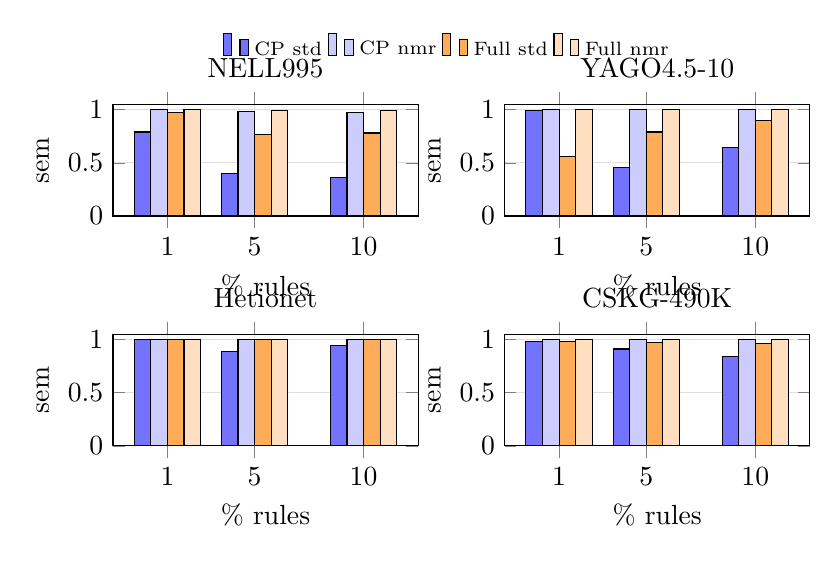
\begin{tikzpicture}
\begin{groupplot}[
  group style={group size=2 by 2, horizontal sep=1.1cm, vertical sep=1.5cm},
  width=0.45\textwidth,
  height=3.0cm,
  ybar,
  enlarge x limits=0.20,
  xlabel={\% rules},
  xtick={1,5,10},
  xmin=0.5,
  xmax=10.5,
  ymin=0,
  ymax=1.05,
  ytick={0,0.5,1.0},
  ylabel={sem},
  yticklabel style={/pgf/number format/fixed},
  grid=both,
  major grid style={draw=gray!25},
  minor grid style={draw=gray!10},
  legend style={
    font=\scriptsize,
    draw=none,
    fill=none,
    % These two lines do the magic:
    at={(1.1, 1.3)}, % (x, y) coordinates relative to the axis
    anchor=south,     % The legend's bottom-center point attaches to those coordinates
    legend columns=4
},
]

% --- NELL995 ---
\nextgroupplot[title={NELL995}]
\addplot+[draw=black, fill=blue!55, bar width=6pt, bar shift=-9pt] coordinates {(1,0.79) (5,0.40) (10,0.36)};
\addplot+[draw=black, fill=blue!20, bar width=6pt, bar shift=-3pt] coordinates {(1,1.00) (5,0.98) (10,0.97)};
\addplot+[draw=black, fill=orange!65, bar width=6pt, bar shift=3pt] coordinates {(1,0.97) (5,0.77) (10,0.78)};
\addplot+[draw=black, fill=orange!25, bar width=6pt, bar shift=9pt] coordinates {(1,1.00) (5,0.99) (10,0.99)};
\legend{CP std, CP nmr, Full std, Full nmr}

% --- YAGO4.5-10 ---
\nextgroupplot[title={YAGO4.5-10}]
\addplot+[draw=black, fill=blue!55, bar width=6pt, bar shift=-9pt] coordinates {(1,0.99) (5,0.46) (10,0.64)};
\addplot+[draw=black, fill=blue!20, bar width=6pt, bar shift=-3pt] coordinates {(1,1.00) (5,1.00) (10,1.00)};
\addplot+[draw=black, fill=orange!65, bar width=6pt, bar shift=3pt] coordinates {(1,0.56) (5,0.79) (10,0.90)};
\addplot+[draw=black, fill=orange!25, bar width=6pt, bar shift=9pt] coordinates {(1,1.00) (5,1.00) (10,1.00)};

% --- Hetionet ---
\nextgroupplot[title={Hetionet}]
\addplot+[draw=black, fill=blue!55, bar width=6pt, bar shift=-9pt] coordinates {(1,1.00) (5,0.89) (10,0.94)};
\addplot+[draw=black, fill=blue!20, bar width=6pt, bar shift=-3pt] coordinates {(1,1.00) (5,1.00) (10,1.00)};
\addplot+[draw=black, fill=orange!65, bar width=6pt, bar shift=3pt] coordinates {(1,1.00) (5,1.00) (10,1.00)};
\addplot+[draw=black, fill=orange!25, bar width=6pt, bar shift=9pt] coordinates {(1,1.00) (5,1.00) (10,1.00)};

% --- CSKG-490K ---
\nextgroupplot[title={CSKG-490K}]
\addplot+[draw=black, fill=blue!55, bar width=6pt, bar shift=-9pt] coordinates {(1,0.98) (5,0.91) (10,0.84)};
\addplot+[draw=black, fill=blue!20, bar width=6pt, bar shift=-3pt] coordinates {(1,1.00) (5,1.00) (10,1.00)};
\addplot+[draw=black, fill=orange!65, bar width=6pt, bar shift=3pt] coordinates {(1,0.98) (5,0.97) (10,0.96)};
\addplot+[draw=black, fill=orange!25, bar width=6pt, bar shift=9pt] coordinates {(1,1.00) (5,1.00) (10,1.00)};

\end{groupplot}
\end{tikzpicture}
\caption{Semantic consistency for AnyBURL rules as a function of the percentage of applied rules (1\%, 5\%, 10\%), extracted from Table~\ref{tab:mat_anyburl_10_30}. Grouped bars (per percentage): CP std, CP nmr, Full std, Full nmr. Values reported as $\sim$1.0 in the table are plotted at 0.99.}
\label{fig:anyburl_inc_trend}
\end{figure}



%%%%%%%%%%%



\begin{table}[ht]
\centering
\scriptsize
\setlength{\tabcolsep}{4pt}
\renewcommand{\arraystretch}{1.15}
\caption{Materialization results for AMIE.}
\label{tab:mat_amie_10_30}

% ===== NELL995 — amie — MAIN =====
\begin{minipage}[t]{0.49\linewidth}
\centering
\textbf{NELL995}\\
\begin{tabular}{c l | r r r r}
\toprule
\% & Metric & L3 & \shortstack{L3\\nmr} & L4 & \shortstack{L4\\nmr} \\
\midrule
1\% & \# applied & 4 & 4 & 139 & 93 \\
1\% & \# target & 5 & 5 & 147 & 147 \\
1\% & \# inc & 20 & 0 & 2908 & 0 \\
1\% & triples & 83 & 63 & 10k & 7.3k \\
1\% & sem & 0.76 & 1.0 & 0.72 & 1.0 \\
1\% & time & 1s & 1s & 8s & 12s \\
\addlinespace
5\% & \# applied & 18 & 18 & 672 & 513 \\
5\% & \# target & 23 & 23 & 731 & 731 \\
5\% & \# inc & 60 & 0 & 9743 & 15 \\
5\% & triples & 1.8k & 1.8k & 36k & 26k \\
5\% & sem & 0.97 & 1.0 & 0.73 & $\sim$1.0 \\
5\% & time & 1s & 2s & 39s & 57s \\
\addlinespace
10\% & \# applied & 40 & 39 & 1227 & 956 \\
10\% & \# target & 45 & 45 & 1462 & 1462 \\
10\% & \# inc & 258 & 40 & 68586 & 30 \\
10\% & triples & 2.4k & 2.2k & 109k & 40k \\
10\% & sem & 0.89 & 0.98 & 0.37 & $\sim$1.0 \\
10\% & time & 2s & 3s & 77s & 111s \\
\bottomrule
\end{tabular}
\end{minipage}%
\hfill
% ===== YAGO4.5-10 — amie — MAIN =====
\begin{minipage}[t]{0.49\linewidth}
\centering
\textbf{YAGO4.5-10}\\
\begin{tabular}{c l | r r r r}
\toprule
\% & Metric & L3 & \shortstack{L3\\nmr} & L4 & \shortstack{L4\\nmr} \\
\midrule
1\% & \# applied & 5 & 4 & 53 & 45 \\
1\% & \# target & 5 & 5 & 74 & 74 \\
1\% & \# inc & 43 & 0 & 1164 & 0 \\
1\% & triples & 22k & 22k & 29k & 28k \\
1\% & sem & $\sim$1.0 & 1.0 & 0.96 & 1.0 \\
1\% & time & 4s & 4s & 36s & 35s \\
\addlinespace
5\% & \# applied & 22 & 16 & 282 & 222 \\
5\% & \# target & 22 & 22 & 366 & 366 \\
5\% & \# inc & 1122 & 0 & 17070 & 0 \\
5\% & triples & 34k & 33k & 79k & 62k \\
5\% & sem & 0.97 & 1.0 & 0.79 & 1.0 \\
5\% & time & 12s & 13s & 181s & 172s \\
\addlinespace
10\% & \# applied & 42 & 36 & 569 & 476 \\
10\% & \# target & 43 & 43 & 732 & 732 \\
10\% & \# inc & 1151 & 0 & 58793 & 0 \\
10\% & triples & 141k & 140k & 255k & 196k \\
10\% & sem & 0.99 & 1.0 & 0.77 & 1.0 \\
10\% & time & 23s & 26s & 367s & 414s \\
\bottomrule
\end{tabular}
\end{minipage}\\[2ex]

\begin{minipage}[t]{0.49\linewidth}
\centering
\textbf{Hetionet}\\
\begin{tabular}{c l | r r r r}
\toprule
\% & Metric & L3 & \shortstack{L3\\nmr} & L4 & \shortstack{L4\\nmr} \\
\midrule
1\%  & \# applied & 1 & 1 & 5 & 5 \\
1\%  & \# target  & 1 & 1 & 5 & 5 \\
1\%  & \# inc     & 26220 & 0 & 0 & 0 \\
1\%  & triples    & 40k & 14k & 1.6k & 1.6k \\
1\%  & sem    &0.34 &1.0 & 1.0 & 1.0 \\
1\%  & time      & 1s & 1s & 1s & 1s \\
\addlinespace
5\%  & \# applied & 3 & 3 & 21 & 20 \\
5\%  & \# target  & 3 & 3 & 21 & 21 \\
5\%  & \# inc     & 26220 & 0 & 2521 & 0 \\
5\%  & triples    & 525k & 499k & 12k & 9.7k \\
5\%  & sem    & 0.95 &1.0 & 0.79 & 1.0\\
5\%  & time      & 2s & 4s & 2s & 2s \\
\addlinespace
10\% & \# applied & 6 & 6 & 40 & 39 \\
10\% & \# target  & 6 & 6 & 41 & 41 \\
10\% & \# inc     & 26220 & 0 & 26282 & 0 \\
10\% & triples    & 957k & 931k & 58k & 32k \\
10\%  & sem    & 0.97&1.0 & 0.55& 1.0\\
10\% & time      & 3s & 7s & 4s & 4s \\
\bottomrule
\end{tabular}
\end{minipage}%
\hfill
% ===== CSKG2 — amie — MAIN =====
\begin{minipage}[t]{0.49\linewidth}
\centering
\textbf{CSKG-490K}\\
\begin{tabular}{c l | r r r r}
\toprule
\% & Metric & L3 & \shortstack{L3\\nmr} & L4 & \shortstack{L4\\nmr} \\
\midrule
1\% & \# applied & 573 & 571 & - & - \\
1\% & \# target & 710 & 710 & - & - \\
1\% & \# inc & 7 & 0 & - & - \\
1\% & triples & 3.7k & 3.7k & - & - \\
1\% & sem & $\sim$1.0 & 1.0 & - & - \\
1\% & time & 64s & 62s & - & - \\
\addlinespace
5\% & \# applied & 2795 & 2792 & - & - \\
5\% & \# target & 3548 & 3548 & - & - \\
5\% & \# inc & 40 & 0 & - & - \\
5\% & triples & 24k & 24k & - & - \\
5\% & sem & $\sim$1.0 & 1.0 & - & - \\
5\% & time & 314s & 296s & - & - \\
\addlinespace
10\% & \# applied & 5590 & 5576 & - & - \\
10\% & \# target & 7096 & 7096 & - & - \\
10\% & \# inc & 260 & 0 & - & - \\
10\% & triples & 56k & 56k & - & - \\
10\% & sem & $\sim$1.0 & 1.0 & - & - \\
10\% & time & 621s & 575s & - & - \\
\bottomrule
\end{tabular}
\end{minipage}%
\end{table}

\begin{table}[]
\centering
\scriptsize
\setlength{\tabcolsep}{3pt}
\renewcommand{\arraystretch}{1.12}
\caption{Materialization metrics for AMIE (`nmr' refers to models with non-monotonic rules), with dis-aggregated inconsistency counts.}
\label{tab:mat_amie_10_30_notot_time}
% ===== NELL995 — amie — BREAKDOWN =====
\begin{minipage}[t]{0.49\linewidth}
\centering
\textbf{NELL995}\\
\begin{tabular}{c l | r r r r}
\toprule
\% & Metric & L3 & \shortstack{L3\\nmr} & L4 & \shortstack{L4\\nmr} \\
\midrule
1\% & \# triples & 83 & 63 & 10k & 7.3k \\
1\% & func & 0 & 0 & 1608 & 0 \\
1\% & dom & 1 & 0 & 381 & 0 \\
1\% & ran & 19 & 0 & 1359 & 0 \\
\addlinespace
5\% & \# triples & 1.8k & 1.8k & 36k & 26k \\
5\% & func & 28 & 0 & 4949 & 15 \\
5\% & dom & 1 & 0 & 1916 & 0 \\
5\% & ran & 39 & 0 & 3587 & 0 \\
\addlinespace
10\% & \# triples & 2.4k & 2.2k & 109k & 40k \\
10\% & func & 226 & 40 & 58894 & 30 \\
10\% & dom & 1 & 0 & 4709 & 0 \\
10\% & ran & 39 & 0 & 44073 & 0 \\
\bottomrule
\end{tabular}
\end{minipage}%
\hfill
\begin{minipage}[t]{0.49\linewidth}
\centering
\textbf{YAGO4.5-10}\\
\begin{tabular}{c l | r r r r}
\toprule
\% & Metric & L3 & \shortstack{L3\\nmr} & L4 & \shortstack{L4\\nmr} \\
\midrule
1\% & \# triples & 22k & 22k & 29k & 28k \\
1\% & func & 43 & 0 & 1138 & 0 \\
1\% & dom & 0 & 0 & 30 & 0 \\
1\% & ran & 0 & 0 & 0 & 0 \\
\addlinespace
5\% & \# triples & 34k & 33k & 79k & 62k \\
5\% & func & 1040 & 0 & 16693 & 0 \\
5\% & dom & 112 & 0 & 447 & 0 \\
5\% & ran & 0 & 0 & 4 & 0 \\
\addlinespace
10\% & \# triples & 141k & 140k & 255k & 196k \\
10\% & func & 1040 & 0 & 57874 & 0 \\
10\% & dom & 141 & 0 & 1527 & 0 \\
10\% & ran & 0 & 0 & 14 & 0 \\
\bottomrule
\end{tabular}
\end{minipage}\\[2ex]

\begin{minipage}[t]{0.49\linewidth}
\centering
\textbf{Hetionet}\\
\begin{tabular}{c l | r r r r}
\toprule
\% & Metric & L3 & \shortstack{L3\\nmr} & L4 & \shortstack{L4\\nmr} \\
\midrule
1\%  & \# triples & 40k & 14k & 1.7k & 1.7 \\
1\%  & func      & -- & -- & -- & -- \\
1\%  & dom       & 26220 & 0 & 0 & 0 \\
1\%  & ran       & 0 & 0 & 0 & 0 \\
\addlinespace
5\%  & \# triples & 525k & 499k & 12k & 9.7k \\
5\%  & func      & -- & -- & -- & -- \\
5\%  & dom       & 26220 & 0 & 2494 & 0 \\
5\%  & ran       & 0 & 0 & 0 & 0 \\
\addlinespace
10\% & \# triples & 957k & 931k & 58k & 32k \\
10\% & func      & -- & -- & -- & -- \\
10\% & dom       & 26220 & 0 & 26278 & 0 \\
10\% & ran       & 0 & 0 & 0 & 0 \\
\bottomrule
\end{tabular}
\end{minipage}%
\hfill
% ===== CSKG2 — amie — BREAKDOWN =====
\begin{minipage}[t]{0.49\linewidth}
\centering
\textbf{CSKG-490K}\\
\begin{tabular}{c l | r r r r}
\toprule
\% & Metric & L3 & \shortstack{L3\\nmr} & L4 & \shortstack{L4\\nmr} \\
\midrule
1\% & \# triples & 3.7k & 3.7k & - & - \\
1\% & func & 0 & 0 & - & - \\
1\% & dom & 0 & 0 & - & - \\
1\% & ran & 7 & 0 & - & - \\
\addlinespace
5\% & \# triples & 24k & 24k & - & - \\
5\% & func & 0 & 0 & - & - \\
5\% & dom & 0 & 0 & - & - \\
5\% & ran & 40 & 0 & - & - \\
\addlinespace
10\% & \# triples & 56k & 56k & - & - \\
10\% & func & 0 & 0 & - & - \\
10\% & dom & 0 & 0 & - & - \\
10\% & ran & 260 & 0 & - & - \\
\bottomrule
\end{tabular}
\end{minipage}%
\end{table}



% Consistency trend plots derived from Table \ref{tab:mat_amie_10_30}
\begin{figure}[t]
\centering
\scriptsize
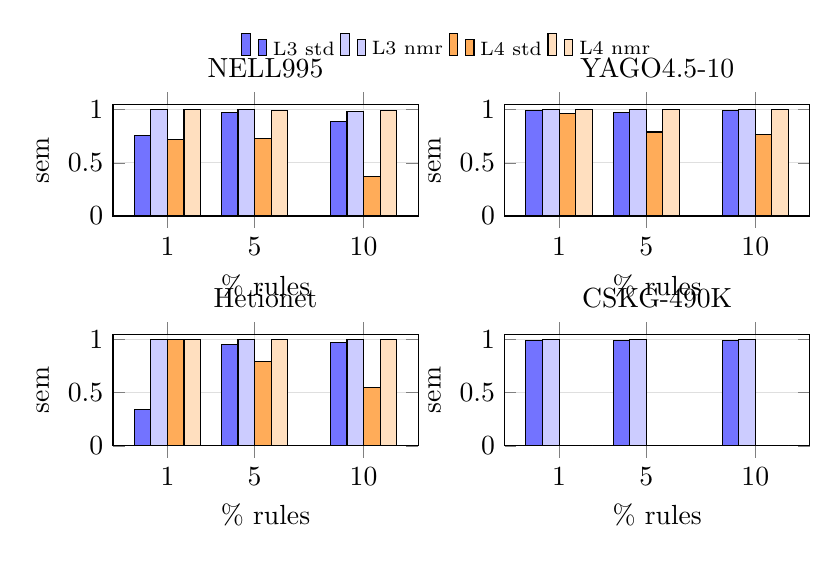
\begin{tikzpicture}
\begin{groupplot}[
  group style={group size=2 by 2, horizontal sep=1.1cm, vertical sep=1.5cm},
  width=0.45\textwidth,
  height=3.0cm,
  ybar,
  enlarge x limits=0.20,
  xlabel={\% rules},
  xtick={1,5,10},
  xmin=0.5,
  xmax=10.5,
  ymin=0,
  ymax=1.05,
  ytick={0,0.5,1.0},
  ylabel={sem},
  yticklabel style={/pgf/number format/fixed},
  grid=both,
  major grid style={draw=gray!25},
  minor grid style={draw=gray!10},
  legend style={
    font=\scriptsize,
    draw=none,
    fill=none,
    % These two lines do the magic:
    at={(1.1, 1.3)}, % (x, y) coordinates relative to the axis
    anchor=south,     % The legend's bottom-center point attaches to those coordinates
    legend columns=4
},
]

% --- NELL995 ---
\nextgroupplot[title={NELL995}]
\addplot+[draw=black, fill=blue!55, bar width=6pt, bar shift=-9pt] coordinates {(1,0.76) (5,0.97) (10,0.89)};
\addplot+[draw=black, fill=blue!20, bar width=6pt, bar shift=-3pt] coordinates {(1,1.00) (5,1.00) (10,0.98)};
\addplot+[draw=black, fill=orange!65, bar width=6pt, bar shift=3pt] coordinates {(1,0.72) (5,0.73) (10,0.37)};
\addplot+[draw=black, fill=orange!25, bar width=6pt, bar shift=9pt] coordinates {(1,1.00) (5,0.99) (10,0.99)};
\legend{L3 std, L3 nmr, L4 std, L4 nmr}

% --- YAGO4.5-10 ---
\nextgroupplot[title={YAGO4.5-10}]
\addplot+[draw=black, fill=blue!55, bar width=6pt, bar shift=-9pt] coordinates {(1,0.99) (5,0.97) (10,0.99)};
\addplot+[draw=black, fill=blue!20, bar width=6pt, bar shift=-3pt] coordinates {(1,1.00) (5,1.00) (10,1.00)};
\addplot+[draw=black, fill=orange!65, bar width=6pt, bar shift=3pt] coordinates {(1,0.96) (5,0.79) (10,0.77)};
\addplot+[draw=black, fill=orange!25, bar width=6pt, bar shift=9pt] coordinates {(1,1.00) (5,1.00) (10,1.00)};

% --- Hetionet ---
\nextgroupplot[title={Hetionet}]
\addplot+[draw=black, fill=blue!55, bar width=6pt, bar shift=-9pt] coordinates {(1,0.34) (5,0.95) (10,0.97)};
\addplot+[draw=black, fill=blue!20, bar width=6pt, bar shift=-3pt] coordinates {(1,1.00) (5,1.00) (10,1.00)};
\addplot+[draw=black, fill=orange!65, bar width=6pt, bar shift=3pt] coordinates {(1,1.00) (5,0.79) (10,0.55)};
\addplot+[draw=black, fill=orange!25, bar width=6pt, bar shift=9pt] coordinates {(1,1.00) (5,1.00) (10,1.00)};

% --- CSKG-490K ---
\nextgroupplot[title={CSKG-490K}]
\addplot+[draw=black, fill=blue!55, bar width=6pt, bar shift=-9pt] coordinates {(1,0.99) (5,0.99) (10,0.99)};
\addplot+[draw=black, fill=blue!20, bar width=6pt, bar shift=-3pt] coordinates {(1,1.00) (5,1.00) (10,1.00)};
\addplot+[draw=black, fill=orange!65, bar width=6pt, bar shift=3pt] coordinates {(1,0.00) (5,0.00) (10,0.00)};
\addplot+[draw=black, fill=orange!25, bar width=6pt, bar shift=9pt] coordinates {(1,0.00) (5,0.00) (10,0.00)};

\end{groupplot}
\end{tikzpicture}
\caption{Semantic consistency for AMIE rules as a function of the percentage of applied rules (1\%, 5\%, 10\%), extracted from Table~\ref{tab:mat_amie_10_30}. Grouped bars (per percentage): L3 std, L3 nmr, L4 std, L4 nmr. (L4 is not available for CSKG-490K and is shown at 0.) Cells with no materialized triples (`-' in the table) and $\sim$1.0 values are plotted at 0 and 0.99 respectively, so a zero-height bar means \emph{either} that nothing was materialized \emph{or} that every materialized triple was inconsistent --- see the table for the distinction.}
\label{fig:amie_inc_trend}
\end{figure}

%%%%%%%%%%%%

\begin{table}[h]
\centering
\caption{Ranking-based LP metrics - CP/L3 and Full/L4 rules.}
\label{tab:metrics_rank}
\begin{tabular}{l | c | c c c | c | c c c}
\toprule
\multicolumn{9}{c}{NELL995} \\
\midrule
& \multicolumn{4}{c|}{CP/L3 rules} & \multicolumn{4}{c}{Full/L4 rules} \\
\cmidrule(lr){2-5} \cmidrule(lr){6-9}
Ruleset & sem@10 & hits@1 & hits@10 & mrr & sem@10 & hits@1 & hits@10 & mrr \\
\midrule
AnyBURL & 0.9927 & 0.1938 & 0.3256 & 0.2409 & 0.9965 & 0.3162 & 0.5318 & 0.3918 \\
AnyBURL nmr & 1.0 & 0.1764 & 0.2911 & 0.2177 & 1.0 & 0.3064 & 0.4907 & 0.3732 \\
AMIE & 0.9897 & 0.1442 & 0.2166 & 0.1703 & 0.9671 & 0.1897 & 0.3230 & 0.2344 \\
AMIE nmr & 1.0 & 0.1404 & 0.2067 & 0.1644 & 1.0 &  0.1839 & 0.3117 & 0.2263 \\
\midrule
\multicolumn{9}{c}{YAGO4.5-10} \\
\midrule
& \multicolumn{4}{c|}{CP/L3 rules} & \multicolumn{4}{c}{Full/L4 rules} \\
\cmidrule(lr){2-5} \cmidrule(lr){6-9}
Ruleset & sem@10 & hits@1 & hits@10 & mrr & sem@10 & hits@1 & hits@10 & mrr \\
\midrule
AnyBURL & 0.9954 & 0.2800 & 0.3389 & 0.3016 & 0.9999 & 0.2566 & 0.2956 & 0.2723 \\
AnyBURL nmr & 1.0 & 0.2731 & 0.3276 & 0.2927 & 1.0 & 0.2562 & 0.2943 & 0.2716 \\
AMIE & 0.9997 & 0.2524 & 0.2873 & 0.2655 & 0.9980 & 0.2797 & 0.3320 & 0.2993\\
AMIE nmr & 1.0 & 0.2517 & 0.2853 & 0.2643 & 1.0 & 0.2780 & 0.3264 & 0.2958\\
\midrule
\multicolumn{9}{c}{Hetionet} \\
\midrule
& \multicolumn{4}{c|}{CP/L3 rules} & \multicolumn{4}{c}{Full/L4 rules} \\
\cmidrule(lr){2-5} \cmidrule(lr){6-9}
Ruleset & sem@10 & hits@1 & hits@10 & mrr & sem@10 & hits@1 & hits@10 & mrr \\
\midrule
AnyBURL  & 0.9999 & 0.0169 & 0.0804 & 0.0382 & 0.9999 & 0.0549 & 0.1310 & 0.0792 \\
AnyBURL nmr & 1.0 & 0.0156 & 0.0797 & 0.0370 & 1.0 & 0.0550 & 0.1310 & 0.0793\\
AMIE & 0.9801 & 0.0283 & 0.1002 & 0.0508 & 0.9902 & 0.0275 & 0.1017 & 0.0506 \\
AMIE nmr & 1.0 & 0.0270 & 0.0992 & 0.0494 & 1.0 & 0.0320 & 0.1063 & 0.0554\\
\midrule
\multicolumn{9}{c}{CSKG-490K} \\
\midrule
& \multicolumn{4}{c|}{CP/L3 rules} & \multicolumn{4}{c}{Full/L4 rules} \\
\cmidrule(lr){2-5} \cmidrule(lr){6-9}
Ruleset & sem@10 & hits@1 & hits@10 & mrr & sem@10 & hits@1 & hits@10 & mrr \\
\midrule
AnyBURL & 0.9658 & 0.0617 & 0.1390 & 0.0874 & 0.9920 & 0.1018 & 0.2255 & 0.1432 \\
AnyBURL nmr & 1.0 & 0.0620 & 0.1363 & 0.0869 & 1.0 & 0.1002 & 0.2191 & 0.1396 \\
AMIE & 0.9759 & 0.1012 & 0.2162 & 0.1397 & -- & -- & -- & --  \\
AMIE nmr & 1.0 & 0.1020 & 0.2167 & 0.1404 & -- & -- & -- & --\\
\bottomrule
\end{tabular}
\end{table}

%%%%%%%%%%%%

\section{Experiments} \label{sec:exp}
We now proceed to illustrate and analyze our empirical experiment setup.
\subsection{Experimental Setup}

\subsubsection{Rule Miners} In principle, our method can be applied on any rule set consisting of closed path rules. To perform an empirical evaluation, we study the effects of schema-based non-monotonic extensions of rules mined using two highly performing rule miners, AnyBurl and AMIE3. As  the methods mine different type of rules and with different criteria, we do not aim to directly compare the two, but intend instead to evaluate the effect of non-monotonic extensions on rule set of different types. We thus use the following settings:
\begin{itemize}
    \item AnyBURL `CP': only cyclic rules, runtime 100s, min confidence: 0.1, min support: 2, rule length: 3 body atoms.
    \item AnyBURL 'Full': fully expressive AnyBURL, runtime 100s (to limit the number of mined rules), min confidence: 0.1, min support: 2, rule length: 3 body atoms.
    \item AMIE3 `L3': min PCA confidence: 0.1, min confidence: 0.1, min support: 2, rule length: 2 body atoms.
    \item AMIE3 `L4': min PCA confidence: 0.1, min confidence: 0.1, min support: 2, rule length: 3 body atoms.
\end{itemize}

\noindent Since AMIE3 performs a full search even on large KGs, we limit the expressivity of its rules for performance reasons. In practice, we excluded any AMIE-mined rules with constants, as well as the longer rules in the case of CSKG2, which our resource could not mine within several days. Despite the trade-off, we obtain in this way closed path rules which are not strictly cyclic, thus integrating a different type of expressivity. We note that this is a standard tractability trade-off acknowledged in recent literature (e.g., frameworks like pyclause\cite{betz_pyclause-simple_2024} similarly limit this expressivity for scalability and comparability).

\subsubsection{Datasets} We extract rules from the following Knowledge Graphs, which are selected as they come with a defined schema, summarized in Table \ref{tab:datasets}. 

\begin{itemize}
    \item NELL995 \cite{xiong_deeppath_2017}, a benchmark knowledge base completion dataset based on the Never-Ending Language Learning (NELL) system.
    \item YAGO4.5-10: YAGO4.5 \cite{suchanek_yago_2024} is a general-purpose Knowledge Graph, which combines entity data from Wikidata with a cleaned, logic-consistent taxonomy primarily derived from schema.org. We build a Link Prediction-oriented version of YAGO4.5, following the same approach of its ancestor YAGO3.10 \cite{dettmers_convolutional_2018}.  We maintain only A-box triples that involve entities appearing themselves in at least 10 other similar triples. 
    \item Hetionet \cite{himmelstein_systematic_2017} a large, heterogeneous biomedical Knowledge Graph that integrates data from a collection of public databases to connect various entities like genes, compounds, and diseases.
    \item CSKG-490K: CSKG-2.0 \cite{dessi_cs-kg_2025} is an automatically generated Knowledge Graph collecting statements from 15 million research papers from the field of Computer Science, based on an expert-defined and evaluated ontology with a high granularity of properties. It provides LP-targeted splits, CSKG-490K is generated by collecting all triples with support $\geq5$.
    \item YAGO4.5-10-flip: ad-hoc variation of the aforementioned dataset to also include inverse-functional properties. Intended for the purposes of this paper and not as a general benchmarking set, further details in Section \ref{sec:flip}.
\end{itemize}

\noindent When computing standard LP metrics, we use the max-aggregation approach for matching rules. In other words, we sort the predictions in lexicographic order according to the confidence of the rules inferring such predictions, with ties broken by the further highest confidence rules. While we are aware of its practical limitations~\cite{ott_rule-based_2023,ott_safran_2021}, it allows to focus on the single rules, which better fits our objective of seeing the effect of extending them with schema-based exceptions.

\subsubsection{Inverse functionality experiment}\label{sec:flip}
While our method can process and detect inverse functionality violations, we could not find datasets that natively included such constraint in their ontology. To verify the behavior of our method, we performed an additional analysis on an adapted version of YAGO4.5-10 where some functional properties are inverted.

We thus generated YAGO4.5-10-flip, a variant of YAGO4.5-10 in which the usable functional properties are replaced by their inverse. The schema of YAGO4.5-10 declares four functional properties, but only two of them are usable for this purpose: \texttt{schema:gender} has nine distinct objects and, once inverted, would return a candidate set of the size of the whole \texttt{Person} population for every query, while \texttt{schema:publisher} occurs in 16 triples and declares blank-node domain and range, which carry no enforceable constraint. We therefore flip \texttt{schema:birthPlace} and \texttt{schema:deathPlace}, which together account for 196,162 triples of the dataset (140,221 and 55,941 respectively).

The construction is a purely directional rewriting: every triple $(s,r,o)$ becomes $(o,r^{-1},s)$ in the training, validation and test splits as well as in the full graph used for materialization, so that the number of triples, the entities and the splits are left unchanged. 
%The inverse properties are minted in the YAGO namespace (\texttt{yago:birthPlaceOf}, \texttt{yago:deathPlaceOf}), as schema.org does not define these terms, and the entity type assertions are copied unchanged, since flipping alters the direction of a statement and not the entities involved. 
In the T-Box, the axioms of the original property are dropped and the inverse is declared an \texttt{owl:InverseFunctionalProperty} with domain and range \emph{swapped} with respect to the original.

Rules are mined on YAGO4.5-10-flip with AnyBURL in the `Full' setting, but with two changes from the configuration used for the main experiments. First, the mining is restricted to the two inverse-functional heads (\texttt{birthPlaceOf}, \texttt{deathPlaceOf}), so that every mined rule is subject to the constraint under study. Second, the confidence threshold is lowered from 0.1 to 0.01 and the snapshot extended from 100s to 300s, yielding 20,562 rules. The lower threshold is necessary because rules with these two heads are individually low-confidence. As a consequence of both deviations, the absolute figures of this experiment are not directly comparable with those of Tables \ref{tab:mat_anyburl_10_30} and \ref{tab:mat_amie_10_30}.


%%%%%%%%
\subsection{Results}

\subsubsection{Materialization results} Tables \ref{tab:mat_anyburl_10_30} and \ref{tab:mat_amie_10_30} report the results for the materialization at thresholds of, respectively, 1\% and 5\% and 10\% sorted rules. `\# applied' and `\# target' refer to respectively the number of rules that produced triples and the number of rules considering the target percentage. `\# inc' refers to the total number of distinct inconsistent triples (Tables \ref{tab:mat_anyburl_10_30_notot_time} and \ref{tab:mat_amie_10_30_notot_time} report the same results with dis-aggregated inconsistency counts), while `\# triples' and `time' intuitively refer to the number of materialized triples and the runtime of the scenario, `sem' is the ratio of triples that are consistent compared to the total number of new triples. Figures \ref{fig:anyburl_inc_trend} and \ref{fig:amie_inc_trend} visualize this latter value.
 
The discrepancy between the target number of rules and the actually applied number of rules has two causes: first, some rules are mined in the training set and when the full graph is re-composed for prediction, rules that have high accuracy and low support might find all their heads already satisfied, becoming unable to predict new triples (for example AMIE L3 and L3 nmr with NELL995 5\%). Second, and more relevant to our method, is that some rules might always predict exceptions and will be stopped by the pruning, thus causing the difference between the scenarios (seen by the difference between the number of rules applied by the standard methods and the nmr methods).

The results show that inconsistencies appear in most scenarios, even if their number relative to the total materialized triples can vary widely (focusing on the top 1\% rules, semantic consistency ranges from 0.56 in YAGO4.5-10 with AnyBURL full rules, to 1.0 in Hetionet). In the datasets where functionality constraint can be evaluated, the related inconsistencies can scale up to considerable percentages also with respect to the materialized triples (see Tables \ref{tab:mat_anyburl_10_30_notot_time} and \ref{tab:mat_amie_10_30_notot_time}), making it particularly problematic if a repair needs to be performed. 

The application of the non-monotonic extensions allows to improve consistency in  all cases, and seems to be particularly effective for the domain/range restrictions, consistently removing them. The remaining influence of out-rule exceptions seems to be largely minimal and we observed it only in one dataset (NELL995). This improvement generally comes at the expense of processing time, both as it requires to parse the schema, and to further process of exception conditions, but the empirical results show that the time increase is generally within the same order of magnitude with respect to the standard condition, with a few exceptions especially for NELL995 and Hetionet CP. In some cases (mostly in YAGO4.5-10), we notice a reduction of rule materialization time, likely due to stopping inconsistency-prone rules with many available (partial) groundings. For example, in YAGO4.5-10 many rules predicting gender are mined. However, candidate subjects often already have an existing gender relation. Any rule that would add additional gender information would either generate inconsistent facts, or not find any viable grounding. With the non-monotonic extensions, such rules are stopped early, allowing the algorithm to move to more promising rules.

Increasing rule expressivity (Anyburl CP to Full) usually, but not consistently, improves the semantic quality, while increasing the rule length (AMIE L3 to L4) causes more unpredictable behaviors, which can be explained as the former operation making the rule set more specific, and the latter extending it. 

\subsubsection{Rank-based metrics} As shown in Table \ref{tab:metrics_rank}, the influence of the non-monotonic extension on hits@k and MRR tends to be negative, but very limited. We attribute this to the quality and precision of high-confidence rules, which likely dominate the results at lower $k$ values: since individual rules can generate multiple predictions for \texttt{(s,p,?)} or \texttt{(?,p,o)} queries, they have the most influence with the top ranks. Given that the sem@10 scores are still not perfect, this shows that while the majority of top-10 predictions are semantically correct, some inconsistent triples are still present. Our extension appears to remove them, but worsens the other LP scores: this suggest that, with standard LP metrics, the inconsistency generating rules could be considered of higher quality despite the certain presence of inconsistencies among the predictions, as the metrics only focus on the relative rank, without addressing the quality of the relevant predictions.\\
\indent Finally, a note on Hetionet and its low-scored performance: compared to other work as e.g.~\cite{betz_supervised_2022}, we do not specifically target a single property, and instead tackle the general task of KG completion, which thus explains the discrepancy on the results. Our interest lies on the semantic consistency of rules with respect to the entire KG schema, and limiting the rules to only predict a specific relation when only domain and range constraints are available would have limited the conclusion we could gain from the results.
\subsubsection{Inverse functionality} Tables \ref{tab:mat_flip_standard} and \ref{tab:mat_flip_nmr} report the materialization of YAGO4.5-10-flip with the rule set restricted to inverse-functional heads, respectively for the standard condition and for the non-monotonic extension. As every mined rule targets \texttt{birthPlaceOf} or \texttt{deathPlaceOf}, every materialized triple is subject to the constraint under study and the counts are directly comparable across the two conditions. Functional and domain violations are zero throughout, since the flipped properties are declared only inverse functional and their domain is satisfied by construction; the residual range violations of the standard condition come from the few rules predicting a subject that is not a \texttt{Person}.

The standard condition violates inverse functionality on a large share of what it infers: 1992 of 2777 triples at the 1\% threshold (71.7\%), 21461 of 40492 at 5\% (53.0\%) and 45407 of 72518 at 10\% (62.6\%), keeping semantic consistency between 0.28 and 0.46. The degradation in quality follows directly from concentrating the rule set on two constrained relations: rules predicting a person for a given place are numerous and mutually inconsistent, whereas in the unrestricted setting, the same rules are diluted among many unconstrained properties.

The non-monotonic extension removes the large majority of these violations, but not all of them. At the 1\% threshold only 8 violations survive; at 5\% and 10\% it removes respectively 96.7\% and 92.6\% of them, raising semantic consistency from 0.46 to 0.96 and from 0.37 to 0.89. The surviving violations grow with the density of the inferred triples, from 1.0\% of the materialized triples at 1\% to 3.6\% at 5\% and 11.1\% at 10\%.

Considering the rule counts roughly a third of the productive rules are stopped entirely as they only predict exceptions. The added cost is modest at this scale, from 368s to 385s at the 10\% threshold.

These residual violations are due to out-rule exceptions. Among the 3340 surviving triples at the 10\% threshold, all originate from 1629 objects receiving two or more distinct subjects from different rules, and none conflicts with a triple already present in the graph. It is the same effect already noted on NELL995, where its influence was minimal; here, as the rule set is deliberately concentrated on inverse-functional heads and the inferred triples are dense over a small set of objects, it becomes the dominant residual source of inconsistency.

Beyond verifying the effect of our method on inverse-functionality constraints, this experiment further highlights a scenario where the out-rule consistency trade-off can be more prominent: in case in which RM is focused only on properties including functional or inverse-functional properties, the number of inconsistencies left by our method might increase, warranting further repair options.

\begin{table}[]
\centering
\scriptsize
\setlength{\tabcolsep}{4pt}
\renewcommand{\arraystretch}{1.12}
\caption{Materialization of YAGO4.5-10-flip with AnyBURL rules restricted to inverse-functional heads, \textbf{standard} condition. `invf', `func', `dom' and `ran' are the inconsistent triples according to, respectively, inverse functionality, functionality, domain and range; `\# inc' is the number of distinct inconsistent triples and `sem' the ratio of consistent triples over the materialized ones. `\# applied', `\# target' and `time' are as in Table \ref{tab:mat_anyburl_10_30}.}
\label{tab:mat_flip_standard}
\begin{tabular}{l | r r r r r r r r r r}
\toprule
\% & \# applied & \# target & \# triples & invf & func & dom & ran & \# inc & sem & time \\
\midrule
1\%  & 155  & 206  & 2777  & 1992  & 0 & 0 & 8   & 2000  & 0.28 & 28s \\
5\%  & 756  & 1029 & 40492 & 21461 & 0 & 0 & 321 & 21778 & 0.46 & 189s \\
10\% & 1530 & 2057 & 72518 & 45407 & 0 & 0 & 355 & 45756 & 0.37 & 368s \\
\bottomrule
\end{tabular}
\end{table}

\begin{table}[]
\centering
\scriptsize
\setlength{\tabcolsep}{4pt}
\renewcommand{\arraystretch}{1.12}
\caption{Materialization of YAGO4.5-10-flip with AnyBURL rules restricted to inverse-functional heads, \textbf{non-monotonic} condition (nmr). Columns as in Table \ref{tab:mat_flip_standard}. The residual `invf' counts are entirely due to out-rule exceptions, i.e. distinct rules predicting different subjects for the same object.}
\label{tab:mat_flip_nmr}
\begin{tabular}{l | r r r r r r r r r r}
\toprule
\% & \# applied & \# target & \# triples & invf & func & dom & ran & \# inc & sem & time \\
\midrule
1\%  & 104  & 206  & 785   & 8    & 0 & 0 & 0 & 8    & 0.99 & 40s \\
5\%  & 519  & 1029 & 19417 & 703  & 0 & 0 & 0 & 703  & 0.96 & 202s \\
10\% & 1035 & 2057 & 30122 & 3340 & 0 & 0 & 0 & 3340 & 0.89 & 385s \\
\bottomrule
\end{tabular}
\end{table}

\subsection{Discussion}
\subparagraph{Consistency vs. Ranking Performance trade-off} Our results show that introducing exceptions can slightly decrease standard LP metrics. However, we argue that this trade-off is in practice unavoidable: our sem@10 results clearly show inconsistencies appearing in most cases in the standard setting, claim which is further verified by the materialization analysis. From a downstream application point of view, materializing the standard rule-set will clearly introduce inconsistencies in the KG, which will require a repairing step that with our method can be avoided or heavily limited. This is can be also contextualized as being close to similar related work \cite{hubert_treat_2024,paulheim_make_2018} which argued for the need of semantic-aware metrics complementary to standard, rank-based ones.

\subparagraph{Remaining Out-Rule Violations} 
Our experiments empirically suggest that the contribution of out-rule exceptions at materialization time is limited. In fact from the \#Inc values in Tables 3,4,6,7 it is possible to notice how, after blocking in-rule and in-graph exceptions, the remaining inconsistencies are often 0 or in rare cases (NELL) only limited to a small percentage (less than 3\%) with respect to the generated triples. In the case of targeted rule mining (Tables 8 and 9), out-rule exceptions can be more prominent, by construction, but the exception-based pruning still heavily reduces them.

When handling out-rule violation, the memory requirements would immediately rise as one needs to track provenance of predictions. Additionally, out-rule violations further involve including considerations about confidence and confidence aggregation: a possible heuristic could consider resolving inconsistencies by including a preference based on higher-confidence rules and blocking lower confidence predictions, but this could only be applied with max-aggregation. It is definitely an open question that warrants further analysis, but we kept it outside of the scope to the paper, as their remaining influence is limited.

\subparagraph{Schema Availability} 
The main bottleneck in expanding our method and evaluating more schema restrictions depends on the limited availability of openly available, large-scale KGs that include curated schemas. While industrial applications increasingly focus on the ontological layer \cite{hofer_construction_2024}, academic benchmarks remain limited. In particular, none of the available KGs allowed us to observe inconsistencies linked to inverse functionality, so we created a version of YAGO4.5-10 to include it, and even in that case, rules with inverse-functional heads remain rare. 

It must be noted that other readily available restrictions under OWL2DL \cite{motik_owl_2012}, like reflexivity and symmetry are also not immediately applicable to exception-based rules: the former is excluded by the principle of object identity, and the latter can only be inconsistent only under close-world assumption, or by applying a chase, both of which we do not currently include. Given this we posit that the three main restrictions that we manage to tackle are nonetheless the most widespread and thus beneficial, while including inverse-functionality exceptions can be of use when available.
%\FloatBarrier
\section{Conclusions}
% \subsubsection{Contributions}
In this paper, we analyzed the effect of schema-based exceptions in rule sets for Link Prediction, with the aim of reducing the number of inconsistencies caused by materialization of standard Horn-like rules. Our method focused on exceptions avoiding in-graph and in-rule violations of domain, range, functionality and inverse-functionality restrictions, implementing them at rule-grounding level, by stopping the DFS search for a given problematic (rule, candidate entity) pair. Our empirical experiments showed that these extensions are sufficient to reduce the number of inconsistent triples, especially when considering domain and range. Functional and inverse-functional inconsistencies are also mostly removed, with some residuals from out-rule exceptions, which increase if only such types of rules are mined. The cost of such improvement is a possible increase in computational time, as the schema must be parsed and further checks are added to the algorithm, but we note that in some cases the computational time was actually improved, likely by stopping high-support inconsistency-generating rules that are instead skipped. 
% We further reported how the quality of the original rule set is actually influenced by the granularity of the schema and the level of curation of the same, with KGs respecting highly curated and granular producing more consistent rules. 

We also show how rank-based metrics are influenced in a limited (but often negative) way by the extension, suggesting that they cannot measure the semantic quality of the predicted triples, as they accept triples even if uniquely predicted by inconsistency-prone rules.
Finally, our method is most effective and more suitable when the rule sets are less expressive and of lower quality. Given that, especially when performing a full search, computational constraints might limit the expressivity of the mined rules, we posit that our method could help reducing the overhead of performing a post-hoc repair of the inferences.
% \subsubsection{Limitations and Future Work}

As discussed, we only included a limited number of restrictions, albeit common, existing in the OWL2~\cite{motik_owl_2012} standard. A possible research direction would be to expand this to include more complex axioms. But our method is also dependent on the presence of a schema (ontology), which is not the common setup for Link Prediction and rarely present in such datasets beyond some simple restrictions. While we argue for the benefits of including semantic information in the pipeline, an alternative approach would be to automatically extract such information from the data, instead of having expert curation in the loop. Finally, we note the need for more semantic-aware LP metrics, either by integration of the available ones, or by the development of alternatives, which would allow to have a more realistic idea of the quality of the methods.

%%
%% Bibliography
%%

%% Please use bibtex, 

\bibliography{references}

\end{document}
